% =============================================================================
%  Dinamica3_Fase1_Diapositiva1.tex — Dinámica 3, Fase 1, Diapositiva 1: el estímulo denso
%  Fondo de pergamino con texto en versos (Canto IX de la Odisea, adaptación).
%  Formato 16:9. Compilar con pdflatex; exportar a PNG con:
%    pdftoppm -png -r 150 -singlefile Dinamica3_Fase1_Diapositiva1.pdf Dinamica3_Fase1_Diapositiva1
% =============================================================================
\documentclass[tikz,border=0pt]{standalone}
\usepackage[utf8]{inputenc}
\usepackage[T1]{fontenc}
\usepackage{ebgaramond}


% ── Paleta ────────────────────────────────────────────────────────────────────
\definecolor{Pergamino}{HTML}{F1EBDD}
\definecolor{PergaminoBorde}{HTML}{DCCFB4}
\definecolor{Fibra}{HTML}{B9A27A}
\definecolor{Tinta}{HTML}{2B2620}

% ── Dimensiones (16:9) ────────────────────────────────────────────────────────
\def\ancho{32}
\def\alto{18}

\begin{document}
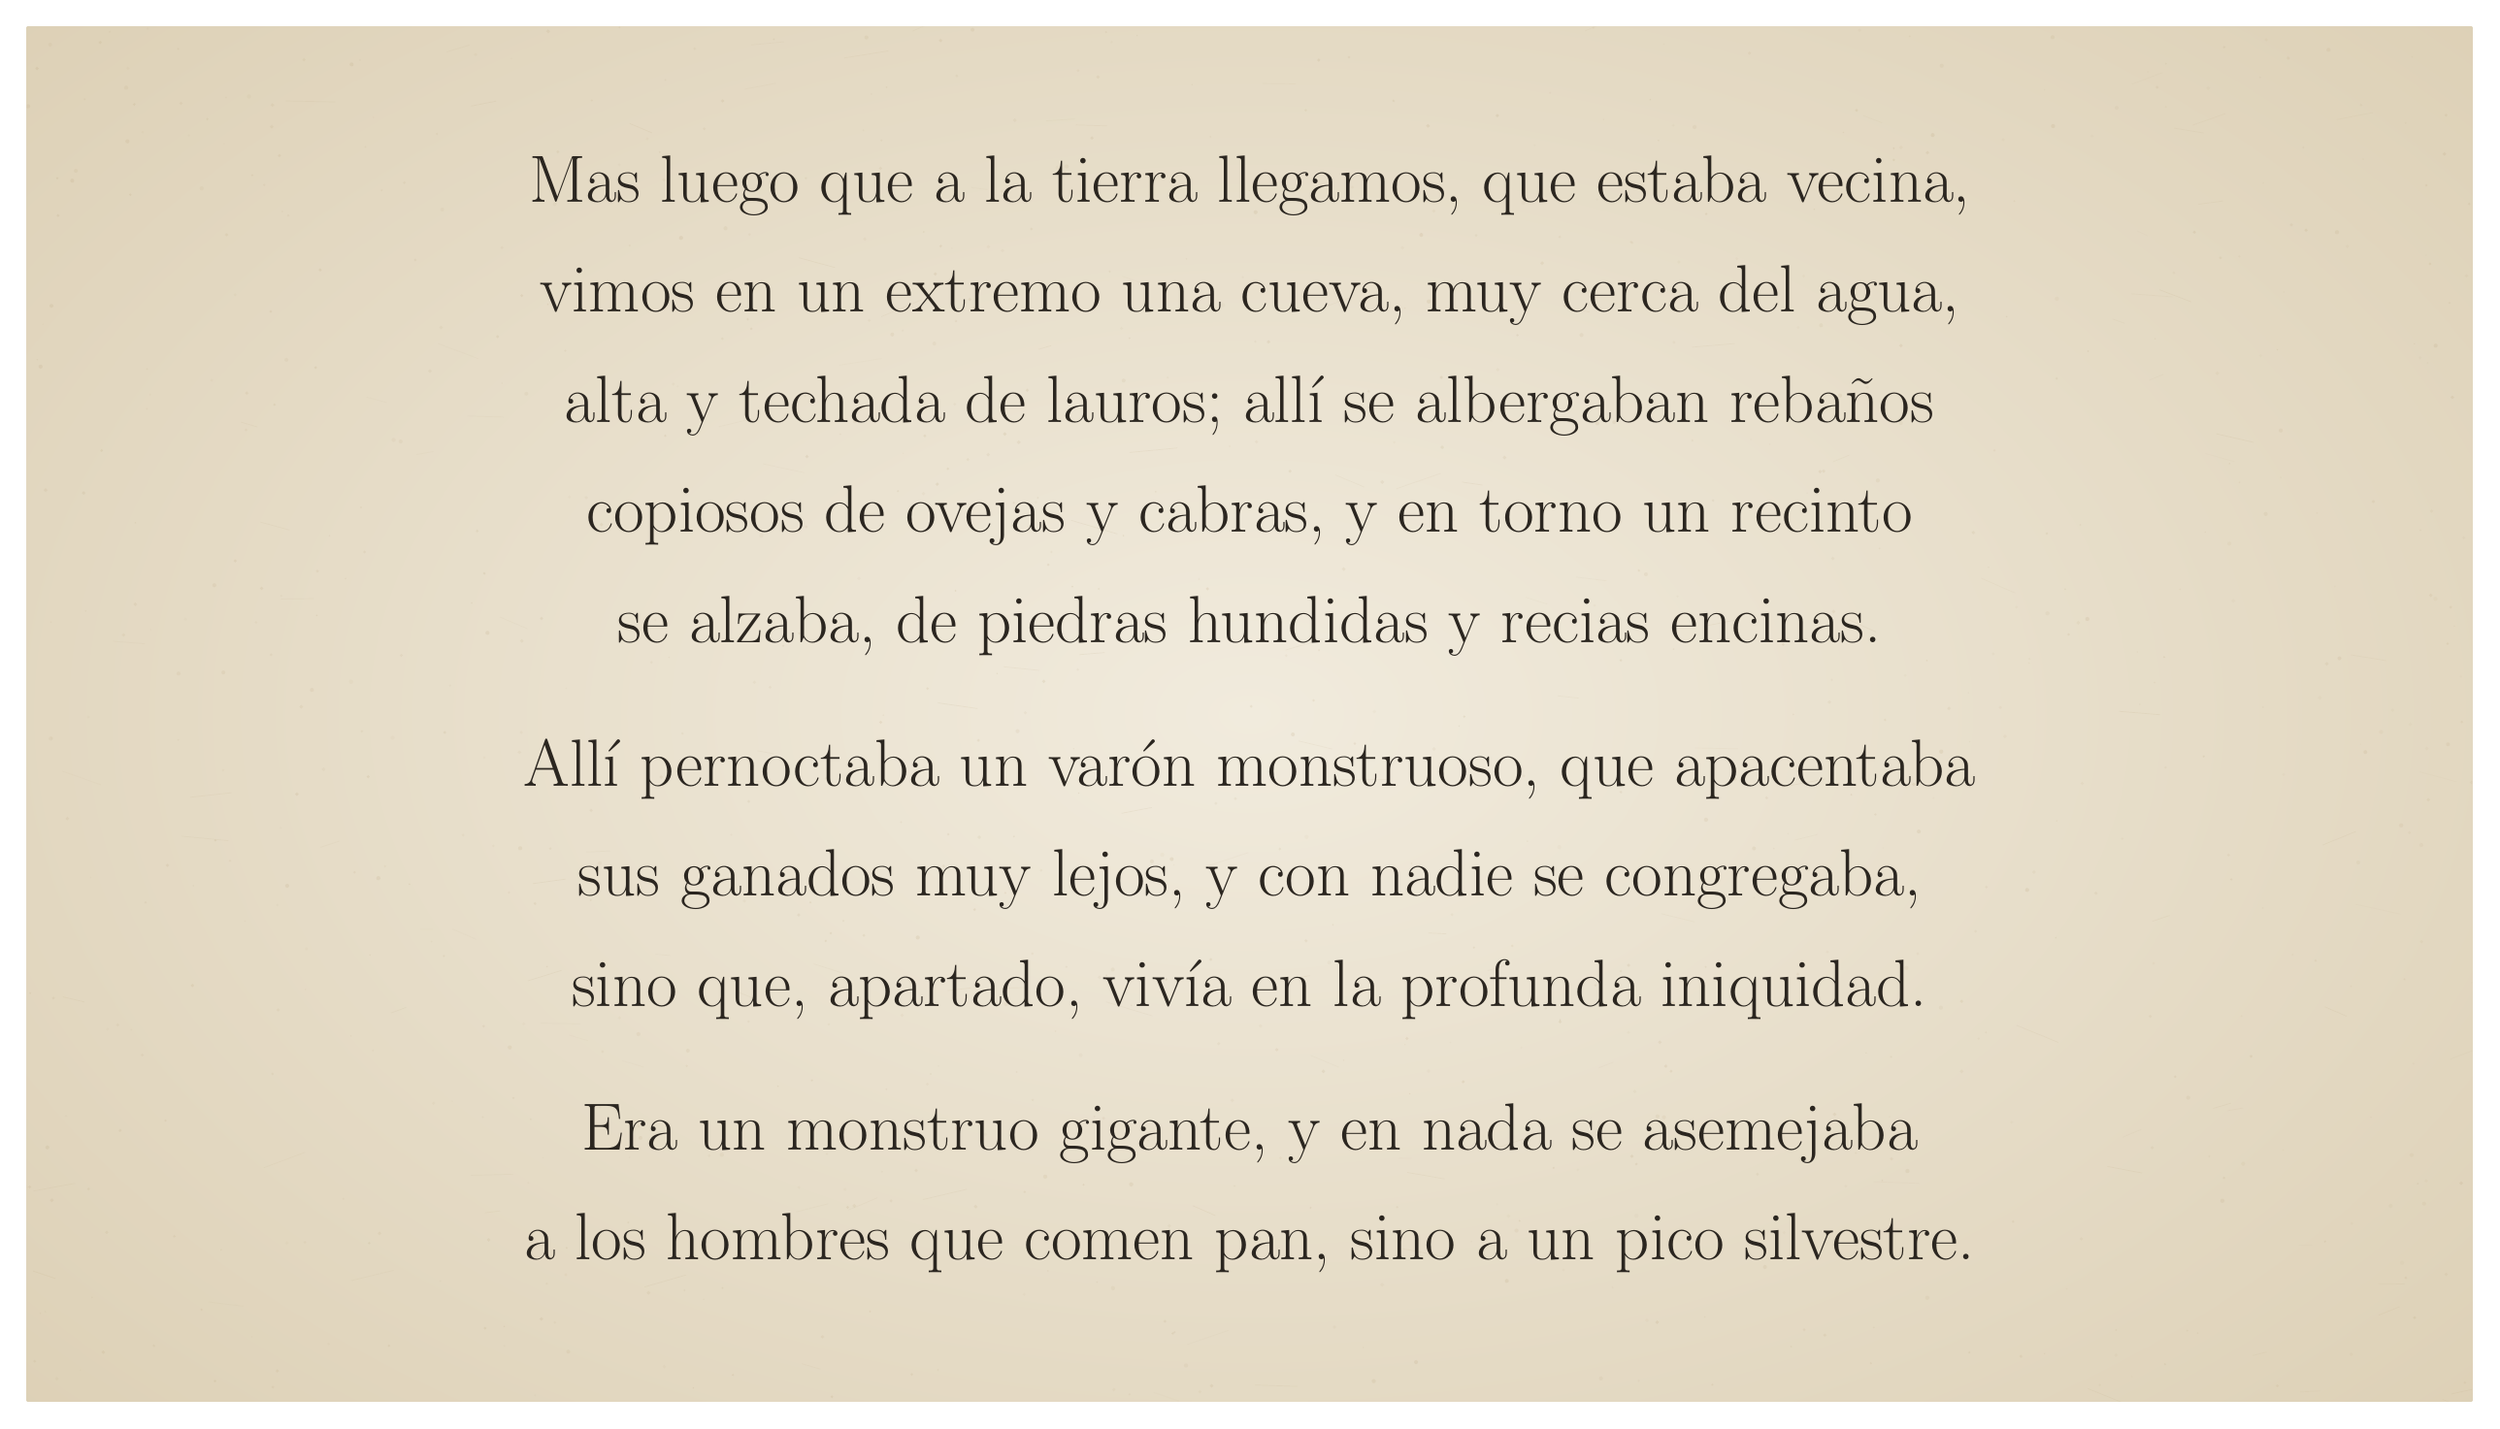
\begin{tikzpicture}
  % Área fija 16:9: nada se dibuja fuera de ella
  \useasboundingbox (0,0) rectangle (\ancho,\alto);
  \clip (0,0) rectangle (\ancho,\alto);

  % Fondo con viñeta: centro claro y bordes más oscuros, como papel envejecido
  \fill[PergaminoBorde] (0,0) rectangle (\ancho,\alto);
  \shade[inner color=Pergamino, outer color=PergaminoBorde]
    (\ancho/2,\alto/2) ellipse [x radius=0.72*\ancho, y radius=0.80*\alto];

  % Textura: fibras y motas finas (semilla fija para resultados reproducibles)
  \pgfmathsetseed{1914}
  \foreach \i in {1,...,900}{
    \pgfmathsetmacro{\x}{rnd*\ancho}
    \pgfmathsetmacro{\y}{rnd*\alto}
    \pgfmathsetmacro{\r}{0.008+0.02*rnd}
    \pgfmathsetmacro{\o}{0.05+0.12*rnd}
    \fill[Fibra, opacity=\o] (\x,\y) circle (\r);
  }
  \foreach \i in {1,...,140}{
    \pgfmathsetmacro{\x}{rnd*\ancho}
    \pgfmathsetmacro{\y}{rnd*\alto}
    \pgfmathsetmacro{\l}{0.15+0.5*rnd}
    \pgfmathsetmacro{\a}{-25+50*rnd}
    \pgfmathsetmacro{\o}{0.04+0.08*rnd}
    \draw[Fibra, opacity=\o, line width=0.25pt, rotate around={\a:(\x,\y)}]
      (\x,\y) -- ++(\l,0);
  }

  % Texto en versos
  \node[text=Tinta, align=center, font=\fontsize{30}{41}\selectfont]
    at (\ancho/2,\alto/2) {%
      Mas luego que a la tierra llegamos, que estaba vecina,\\
      vimos en un extremo una cueva, muy cerca del agua,\\
      alta y techada de lauros; allí se albergaban rebaños\\
      copiosos de ovejas y cabras, y en torno un recinto\\
      se alzaba, de piedras hundidas y recias encinas.\\[0.55em]
      Allí pernoctaba un varón monstruoso, que apacentaba\\
      sus ganados muy lejos, y con nadie se congregaba,\\
      sino que, apartado, vivía en la profunda iniquidad.\\[0.55em]
      Era un monstruo gigante, y en nada se asemejaba\\
      a los hombres que comen pan, sino a un pico silvestre.%
    };
\end{tikzpicture}
\end{document}
